\documentclass[]{article}
\usepackage{authblk}

%opening
\title{EM-Driven GMM Optimization for the Randall Dataset: Rooting and Recall}
\author[1]{Prabhav Kalaghatgi}
\affil[1]{Independent Researcher, Hyderabad, India}

\begin{document}
	
	\maketitle
	
	\begin{abstract}
		
	\end{abstract}
	
	\section{Introduction}	
		\subsection*{Related work}
		\subsection*{Claims to clarify}
	\section{Results}		
		\subsection{Impact of initial parameters on final log likelihood scores}
		\begin{figure}[htbp]
			\centering
			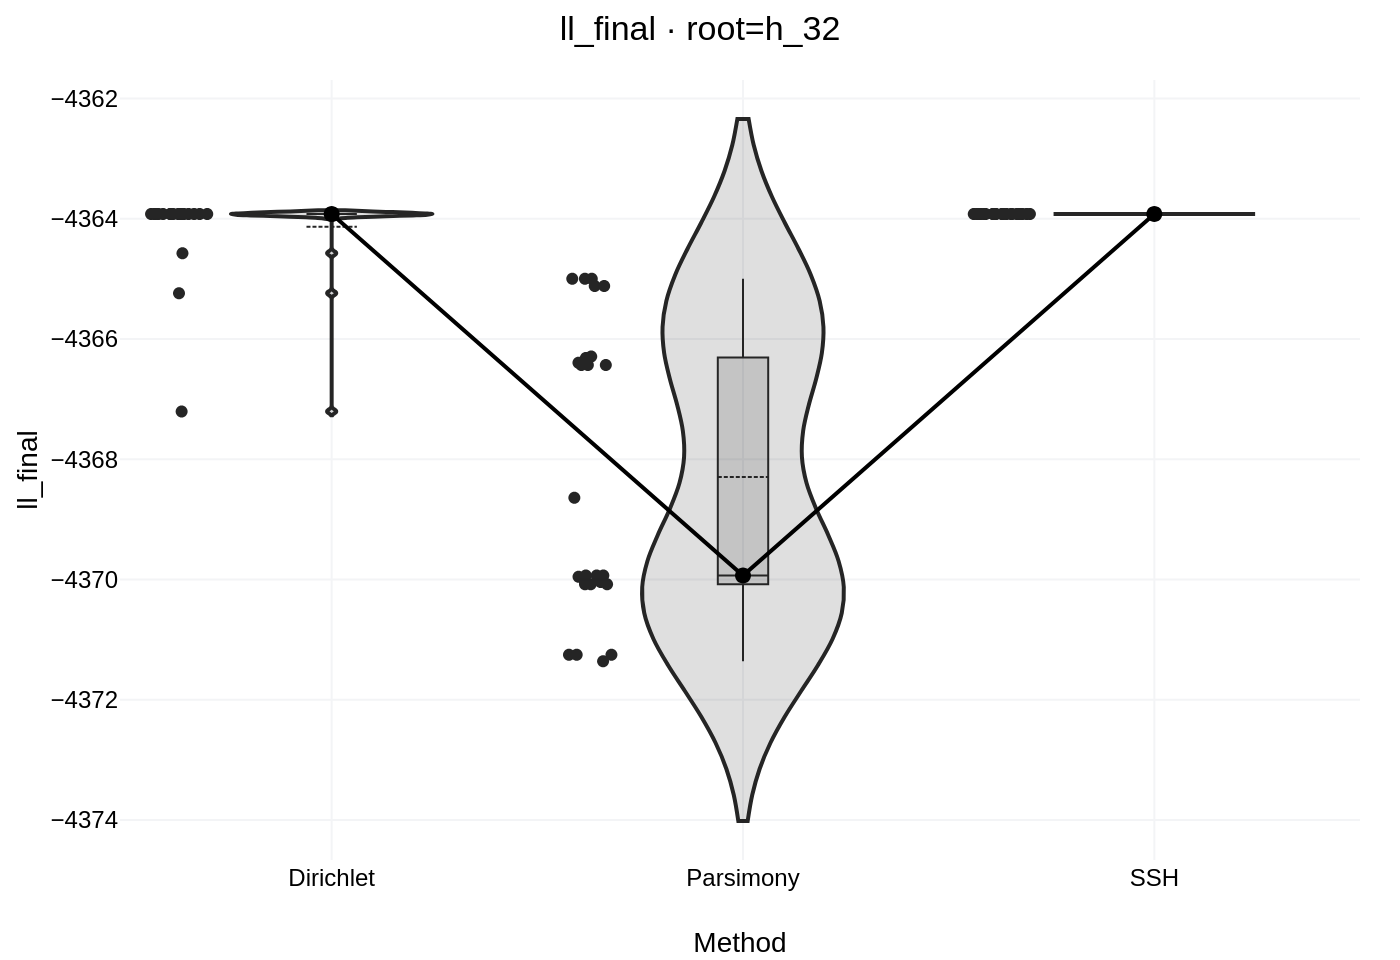
\includegraphics[width=0.8\textwidth]{"/home/pk/projects/prabhavk.github.io/public/figures/wasm-1756002951415__violin__ll_final_violin__t20250824_225734Z.png"}
			\caption{This is the caption describing the figure.}
			\label{fig:my_label}
		\end{figure}
		
		\subsection{Distribution of optimization scores across root locations}
		\begin{figure}[htbp]
			\centering
			\includegraphics[width=0.8\textwidth]{path/to/your/figure.png}
			\caption{This is the caption describing the figure.}
			\label{fig:my_label}
		\end{figure}
		
		\subsection{Wilcoxon-Mann-Whitney tests for difference in log likelihood scores}
			\subsubsection{Initialization Method}
			\subsubsection{Change across root locations}				
		\subsection{Significance of recall values}
		
	\section{Methods}		
		\subsection{EM for fixed topology and root}
		\subsection{Parameter initialization}
		\subsubsection{Dirichlet}
		\subsubsection{Parsimony}
		\subsubsection{SSH}
		\subsection{Statistical tests}
		\subsection{Reproducibility of results}
	\section{Discussion}	
	
\end{document}


